% ISS presentation template
%
% Change history:
% 24.06.2010    J�rgen Ruoff        Initial creation
% 01.07.2010    Patrick H�cker      Generalization
% 02.07.2010    Patrick H�cker      Adjustment
% 15.11.2010    Patrick H�cker      Improvements
% 20.05.2011    Patrick H�cker      Add presentation type
% 06.01.2012	P. Hermannst�dter 	Adapted to ISS, small mods

% Insert your name here
\newcommand{\presenter}{Zhuowei Han}
\newcommand{\presentershort}{Z.Han}
\newcommand{\presenteremail}{} 		% can be accessed using \presenteremail

% Insert presentation title here
\newcommand{\presentationtitle}{Learning Deep Architectures for Pattern Recognition}
\newcommand{\shortpresentationtitle}{Deep Learning}

% Insert type of presentation here (or comment line), probably one of:
% Mitarbeitervortrag, Bachelor-Arbeit, Master-Arbeit, Bachelor thesis, Master thesis
\newcommand{\presentationtype}{---An introduction to Deep Neural Networks---}

% Insert presentation date here
\newcommand{\presentationdate}{05.06.2014}

% Uncomment the following line, if you write in English
%\newcommand{\lang}{german}

% Uncomment the following line, if you want to create handouts (setting to false does not work!)
% \newcommand{\handoutmode}{true}

% Load beamer class using LSS style
% Default \lang to ngerman
\ifx\lang\undefined
	\newcommand{\lang}{ngerman}
\fi

% Set \handout dependant on \handoutmode
\ifx\handoutmode\undefined
	\newcommand{\handout}{}
\else
	\newcommand{\handout}{handout}
\fi

% Make additional colors available
\PassOptionsToPackage{x11names}{xcolor}

% Load the beamer class, set the presentation data and use the LSS layout
\documentclass[\lang,\handout]{beamer}
\author[\presentershort]{\presenter}
\title[\shortpresentationtitle]{\presentationtitle}
\ifx \presentationtype \undefinded
\else
	\subtitle{\presentationtype}
\fi
\date{\presentationdate}
\institute{Institut f�r Signalverarbeitung\\und Systemtheorie\\\vspace{1em}Universit�t Stuttgart}
\usetheme[alternativetitlepage=true,% Use the fancy title page.
          titlepagelogo=isslogocolor,% Logo for the first page.
          watermark=isslogocolor,% Watermark used in every page.
          watermarkheight=25px,% Height of the watermark.
          ]{LSS}

% Grays uncovered objects instead of making them invisible; comment to make uncovered objects invisible
\setbeamercovered{transparent}

% Set work to presentation to not get blue hyperlinks
\newcommand{\work}{presentation}

% Input general definitions and loading of packages which can be shared with the thesis.
% Comment this line if you want to decide yourself which packages should be loaded.
% \def\me{Patrick H�cker}

% this is needed to get more resources to TeX - otherwise not all packages work at the same time
\usepackage{etex}

% erm�glicht ein if-then-else in LaTeX z. B. um Pakete variabel einzubinden
\usepackage{xifthen}
% \newcommand{\ifthen}[1]{\ifthenelse{#1}{}} % It does not work (behaviour is wrong)

% Load language specific things. Always load german, too, to get things like the long name of LSS correctly.
\ifx\lang\undefined
	\newcommand{\lang}{ngerman}
\fi
\ifthenelse{\equal{\lang}{german}}{
	\renewcommand{\lang}{ngerman}
}{}

\ifthenelse{\not\equal{\lang}{ngerman}}{
	\usepackage[ngerman,\lang]{babel}
}{
	\usepackage[\lang]{babel}
}

% damit man Umlaute direkt eingeben kann und diese erkannt werden (sp�ter auf utf8 umsteigen).
\usepackage[x-iso-8859-1]{inputenx}

% Umlaute werden als eine Einheit angesehen -> richtige Trennung und korrekt ins PDF eingebunden;
\usepackage[T1]{fontenc}

% Enth�lt gewisse Sonderzeichen wie z. B. Bullets
\usepackage{textcomp}

% Allow more set symbols (does not replace amsmath symbols if included before amsmath)
\usepackage[bbgreekl]{mathbbol}

% Schaltet AMS-Befehle, Schriftzeichen und Symbole frei (Mathepaket)
% Allow bold uppercase greek letters using the boldsymbol command
\usepackage{amsmath}
\usepackage{amsfonts}
\usepackage{amssymb}

% Allows bold italic uppercase letters
\usepackage{fixmath}



%Erlaubt den Seitenumbruch in Formeln, auch wenn er nach M�glichkeit vermieden wird
\allowdisplaybreaks[4]

% Enables fraction of the form a/b (with a nice slash)
\usepackage{nicefrac}

% Bindet die standardm��ig genutzten Times-Fonts ein (muss nach amsmath eingebunden werden)
% \usepackage{txfonts}

% Uses the Latin Modern font
\usepackage{lmodern}

% erm�glicht die aufrechte Schreibung griechischer Buchstaben
\usepackage{upgreek}

%erm�glicht das Einbinden von EPS-Dateien
\usepackage{graphicx}

%Das nachtr�gliche �ndern von Texten und Anpassen der Schriftart in EPS-Dateien beim Einbinden
\usepackage{psfrag}

%erm�glicht farbigen Text
\usepackage[x11names]{xcolor}

%erm�glicht farbige Tabellenhintergr�nde
\usepackage{colortbl}

% tikz is a cool drawing package using pgf
\usepackage{tikz}

\usetikzlibrary{3d,arrows,automata,backgrounds,calc,calendar,chains,decorations,decorations.footprints,decorations.fractals,decorations.markings,decorations.pathmorphing,decorations.pathreplacing,decorations.shapes,decorations.text,er,fadings,fit,folding,matrix,mindmap,patterns,petri,plothandlers,plotmarks,positioning,scopes,shadows,shapes.arrows,shapes.callouts,shapes,shapes.gates.logic.IEC,shapes.gates.logic.US,shapes.geometric,shapes.misc,shapes.multipart,shapes.symbols,through,topaths,trees}

% pgfplots enables the simple creation of plots from data points (eg. generated by matlab2tikz.m)
\usepackage{pgfplots}

% save every tikz plot as a pdf file (see package documentation of pgfplots)
% \usepgfplotslibrary{external}
% \tikzexternalize{ the main file name }

% If you want to print on a different size, use this package temporally
% \usepackage{pgfpages}
% \pgfpagesuselayout{resize}[a3paper]

% set PGF's decimal separator to comma for german documents
\ifthenelse{\equal{\lang}{ngerman}}{
	\pgfkeys{/pgf/number format/.cd, set decimal separator={{{,}}}}
}{}

% damit kann man Diagramme und Funktionen zeichnen
% \usepackage{pstricks,pst-plot,pst-node}
%\usepackage{pstricks-add}

% Zugriff auf gnuplot aus LaTeX heraus (erfordert -shell-escape bei latex-Aufruf)
% \usepackage{gnuplottex}

%\usepackage{multicol}

% Introduces \vref, a command which adds the page to the reference if necessary
\usepackage{nameref}
\usepackage{varioref}

\ifthenelse{\equal{\work}{thesis} \OR \equal{\work}{paper}}{
	\ifthenelse{\equal{\version}{computer}}{
		\def\colortype{color}
	}{}
	\ifthenelse{\equal{\version}{print}}{
		\def\colortype{black}
	}{}

	% Macht Links und Referenzen farbig und entfernt h�ssliche K�stchen drumherum
	% Hyperlinks blau ('color') (=PC-Version) oder schwarz ('black') (=Druckversion)
	\ifthenelse{\equal{\colortype}{color}}{
		\usepackage[breaklinks=true,colorlinks,linkcolor=blue]{hyperref}
	}{
		\usepackage[breaklinks=true]{hyperref}
	}
}
{
	\usepackage{hyperref}
}

% Makes the boolean ifpdf available to check if LaTeX is directly generating a PDF file


\usepackage{ifpdf}

\ifpdf
\else
	% Sorgt daf�r, dass \url-Befehl automatische Umbr�che unterst�tzt (macht Probleme mit pdflatex)
	\usepackage{breakurl}
\fi

% Erm�glicht Abbildungen, die vom Text umflossen werden
% (zwei unterschiedliche Ans�tze, haben wohl beide Nachteile)
% \usepackage{floatflt}
\usepackage{wrapfig}

% Setzt manche Bildunterschriften n�her ans Bild heran, was sch�ner aussieht
\usepackage[hang]{caption}

% mehrere kleine Tabellen oder Grafiken aneinander anordnen (muss nach caption eingebunden werden)
%\usepackage{subfig}

%\usepackage{subfloat}

% Sauber formatierte Quellcode-Umgebung zur Verf�gung stellen
\usepackage{listings}

% Erm�glicht Tabellen, deren Gesamtbreite eingestellt werden kann, wobei eine Spalte �brigen Platz bekommt
\usepackage{tabularx}

% Erm�glicht Tabellen, deren Gesamtbreite eingestellt werden kann, wobei �briger Platz prozentual aufgeteilt wird
\usepackage{tabulary}

% Erstellt sch�nere Tabellen, wobei vertikale Linien nicht mehr benutzt werden d�rfen
\usepackage{booktabs}

% Erm�glicht Tabellenzellen die Ausdehnung �ber mehrere Zeilen
\usepackage{multirow}

% Writes an additional file to enable backward synchronisation between PDF and LaTeX
% "pdfsync uses extremely sensible code. You should not use pdfsync on final documents because
% it can change the layout rather significantly", yep, I hit a bug
% \usepackage{pdfsync}

% Erm�glicht das hinzuf�gen von fixme-Kommentaren, auch als \todo
\usepackage{fixme}
\newcommand{\todo}[1]{\fxwarning{#1}}
%\usepackage[inline,\status]{fixme}

% Ist f�r die �bergangsphase zu pdflatex sinnvoll, weil dann auch eps-Grafiken eingebunden werden k�nnen
%\usepackage{epstopdf}

% Abk�rzungsverzeichnis erstellen und konfigurieren
%\usepackage[german,intoc]{nomencl}
%\renewcommand{\nomname}{Abk�rzungsverzeichnis}
%\let\abbrev\nomenclature
%\setlength{\nomlabelwidth}{.15\hsize}
%\makenomenclature

% Stellt \doublespacing, \onehalfspacing und \singlespacing zur Verf�gung
\usepackage{setspace}

% Allows putting two images on top of each other
% \usepackage[percent]{overpic}

% The savetrees package packs as much text as possible onto each page
% \usepackage{savetrees}

% Stellt das Kommando \extrarowheight f�r das glossaries-Paket zur Verf�gung
\usepackage{array}

% allows usage of \degree
\usepackage{gensymb}

% Abk�rzungen
% Sets
\newcommand{\Z}{\mathbb{Z}}
\newcommand{\N}{\mathbb{N}}
\newcommand{\Q}{\mathbb{Q}}
\newcommand{\R}{\mathbb{R}}
\newcommand{\C}{\mathbb{C}}

% differentiation
\newcommand{\del}{\partial}
\newcommand{\derivate}[2]{\frac{\del #1}{\del #2}}
\DeclareMathOperator{\dif}{d}
\DeclareMathOperator{\gradlong}{grad}
\DeclareMathOperator{\grad}{\bigtriangledown}

% statistics
\newcommand{\erw}[1]{\operatorname{E}\left(#1\right)}
\DeclareMathOperator{\E}{E}
\DeclareMathOperator{\prop}{P}
\DeclareMathOperator{\Var}{Var}
\DeclareMathOperator{\Cov}{Cov}
\DeclareMathOperator{\Bias}{Bias}
\DeclareMathOperator{\CRB}{CRB}

% linear algebra
\newcommand{\mat}[1]{\mathbf{#1}}
%\newcommand{\mat}[1]{\boldsymbol{#1}}
\newcommand{\Tr}[1]{\mathrm{Tr}\left( #1 \right)} %deprecated
\newcommand{\tr}[1]{\mathrm{tr}\left( #1 \right)}
\newcommand{\rang}[1]{\mathrm{rang}\left( #1 \right)}
\newcommand{\diag}[1]{\mathrm{diag}\left( #1 \right)}
\newcommand{\pinv}[1]{#1^{\dagger}}
\newcommand{\trans}[1]{#1^{\mathrm{T}}}
\newcommand{\hermitian}{\mathrm{H}}
\newcommand{\herm}[1]{#1^\mathrm{H}}
\newcommand{\konj}[1]{#1^{\mathrm{*}}}
\newcommand{\est}[1]{\hat{#1}}
\newcommand{\abs}[1]{\left\lvert#1\right\rvert}
\newcommand{\norm}[1]{\left\lVert#1\right\rVert}

% german abbreviations
\newcommand{\zB}{\mbox{z.\,B. }}
\newcommand{\iA}{\mbox{i.\,A. }}
\newcommand{\deha}{\mbox{d.\,h.\ }}
\newcommand{\oae}{\mbox{o.\,�.\ }}
\newcommand{\uae}{\mbox{u.\,�.\ }}
\newcommand{\oBdA}{\mbox{o.\,B.\,d.\,A. }}
\newcommand{\OBdA}{\mbox{O.\,B.\,d.\,A. }}
\newcommand{\ggf}{\mbox{ggf.\ }}
\newcommand{\vgl}{\mbox{vgl.\ }}
\newcommand{\evtl}{\mbox{evtl.\ }}
\newcommand{\bzw}{\mbox{bzw.\ }}
\newcommand{\bspw}{\mbox{bspw.\ }}
\newcommand{\ca}{\mbox{ca.\ }}

% english abbreviations
\newcommand{\eg}{\mbox{e.g.\ }}
\newcommand{\ie}{\mbox{i.e.\ }}

% quotes
\newcommand{\gq}[1]{\glq#1\grq}
\newcommand{\gqq}[1]{\glqq#1\grqq}
\newcommand{\eq}[1]{`#1'}
\newcommand{\eqq}[1]{``#1''}


% functions
\newcommand{\e}[1]{\operatorname{e}^{\,#1}}
\newcommand{\argmax}[2]{\underset{#1}{\operatorname{argmax}}\left( #2 \right)}
\newcommand{\argmaxima}[2]{\underset{#1}{\operatorname{argmaxima}}\left( #2 \right)}
\newcommand{\argmin}[2]{\underset{#1}{\operatorname{argmin}}\left( #2 \right)}
\DeclareMathOperator{\arc}{arc}
\DeclareMathOperator{\sinc}{sinc}
\DeclareMathOperator{\ggT}{ggT}
\DeclareMathOperator{\kgV}{kgV}
\DeclareMathOperator{\lcm}{lcm}

% symbols
% \newcommand{\degree}{\ensuremath{^\circ}}
\newcommand{\entspricht}{\mathrel{\hat{=}}}
\newcommand{\sollgleich}[0]{\overset{!}{=}}
\newcommand{\help}{\textcircled{\scriptsize{?}}}

% general
\newcommand{\op}[1]{\operatorname{#1}}
\newcommand{\smtext}[1]{{\scriptscriptstyle\text{#1}}}
%Zeilenumbruch mit eineinhalbzeiligem Abstand
\newcommand{\br}{\vspace{0.6em}\newline} %entspricht etwa \par\smallskip, geht aber auch in captions
\newcommand{\unit}[2]{\ensuremath{#1}\,\ensuremath{\mathrm{#2}}}
% \newcommand{\definition}[1]{\textit{#1}}
\newcommand{\includeplot}[1]{\centering\includegraphics{parent/Plots/#1.eps}}
\newcommand{\link}[1]{\href{#1}{\url{#1}}}
\newcommand{\shortlink}[1]{\href{#1}{#1}}
\newcommand{\mailto}[1]{\href{mailto:#1}{#1}}
\newcommand{\textlink}[2]{\href{#2}{\url{#1}}}
\newcommand{\vecfun}[2]{#1\hspace{-0.1em}\left(\vec #2\right)}
\newcommand{\equal}[1]{\overset{\text{#1}}{=}}
\newcommand{\matlab}{\textsc{Matlab}\raisebox{1ex}{\tiny{\textregistered}} }

% renews
\renewcommand{\inf}{\infty}
\renewcommand{\matrix}[1]{\mathbf{#1}}
\renewcommand{\j}{\mathrm{j}}
\renewcommand{\gcd}[0]{\operatorname{gcd}}
\renewcommand{\-}{\,--\,}


% Definiert den Befehl \writetofile, der als erstes Argument den Dateinamen und als zweiten Befehl den zu schreibenden Text erwartet
\newcommand{\writetofile}[2]{
% Erstelle Variable outfile
\newwrite\outfile
%�ffne Datei mit Handle outfile
 \immediate\openout\outfile=#1
%Schreibe in Datei
 \immediate\write\outfile{#2}
%Schlie�e Datei
\immediate\closeout\outfile
}

\newcommand{\readfromfile}[1]{
\newread\infile
\immediate\openin\infile=#1
\immediate\read\infile to \tempXBE
\immediate\closein\infile
\tempXBE
}


% \newcommand{\dotsnewline}{\mydotfill\,\linebreak.}

% Allgemeinerer Ansatz als Paket nomencl um mehrere Abk�rzungs-/Symbolverzeichnisse zu erstellen
% Glossary "acronym" wird vordefiniert und Glorraries kommen in Inhaltsverzeichnis (toc)
% einsetzbar: toclike2, toclike3
%\usepackage[acronym,toc,style=toclike3acronym]{glossaries}
% deactivate toclike3acronym temporally due to squeeze upgrade

% Deactivated here and activated in main document, as makeglossaries does not work otherwise (WTF?)
% \usepackage[acronym,toc,style=listdotted]{glossaries}

% Abschlie�ender Punkt in jeder Zeile wird weggelassen
% \renewcommand{\glspostdescription}{}
% L�sst Leerzeile bei Anfangsbuchstabenwechsel in den Verzeichnissen weg
% \renewcommand{\glsgroupskip}{}

% \newcommand{\newacronymdots}[2]{\newglossaryentry{#1}{type=\acronymtype, name={#1}, description={#2}, text={#1}, first={#2 (#1)}, plural={#1s}, firstplural={#2s (#1s)}, symbol={\dotsnewline}}}


% \newcount\boolcounter
% \boolcounter=1
% \advance\boolcounter by 1
% erm�gliche Kennzeichnung eines Akronyms im Text durch \acronym{was}
%%%\newcommand{\acronym}[1]{\acr{#1}}
% \newcommand{\acronym}[1]{\gls{#1}}
% \let\acronym\gls
% \newcommand{\acronym}[1]{#1}
%\newcommand{\acronymnolink}[1]{\protect\acr*{#1}}
% erm�glicht die Benutzung eins Akronyms mit beliebigem Text (Argument #2)
% \newcommand{\acronymtext}[2]{\glslink{#1}{#2}}
% erm�glicht das Benutzen eines Akronyms, ohne dass die ausgeschriebene Version (dieses Mal) verwendet wird
% \newcommand{\acronymshort}[1]{\glslink{#1}{#1}}
% Verwendet ein Akronym ohne einen Link zu setzen (geht nicht in floating-Umgebungen)
%\newcommand{\acronymnolink}[1]{#1\glsadd{#1}}
% erm�gliche Definition eines Akronyms in akronyme.tex durch \defineacronym{was}{wie}
% \newcommand{\defineacronym}[2]{\newacronym{#1}{#1}{#2}}
% \newcommand{\defineacronym}[2]{}
% \newcommand{\defineacronymdots}[2]{\newacronymdots{#1}{#2}}
%Sorgt daf�r, dass man "\acronym{DoS}[-Angriff]" schreiben kann und dann automatisch "DoS-Angriff (Denial of Service)"
%geschrieben wird, bzw. "DoS-Angriff", je nachdem, ob es das erste Mal ist oder nicht
% \defglsdisplayfirst[acronym]{#3#4 (#2)}
% analog zu Akronymen: \definevar legt Symbol an, \var referenziert dieses
% \let\var\gls
% \newcommand{\var}[1]{#1}
% \newcommand{\var}[1]{\ifodd\boolcounter{%
% \protect\gls*{#1}%
% }\else%
% \text{\gls{#1}}\fi%
% }
%\newcommand{\varshort}[1]{\text{\glslink{#1}}\text{#1}}
%\newcommand{\varquiet}[1]{\glsadd{#1}}
%\newcommand{\definevar}[3]{\newglossaryentry{#1}{name=\ensuremath{#2},description={#3},sort=#1}}
\newcommand{\definevar}[4]{\newglossaryentry{#2}{name=\ensuremath{#3},description={#4},sort=#1}}
% \newcommand{\definevar}[4]{}
%\newcount\varcounter
%\varcounter=1
%\newcommand{\definevar}[3]{\definevariable{#1}{#2}{\arabic\varcounter #3}{\arabic\varcounter}}%{\arabic\varcounter}\advance\varcounter by 1}
%\newcommand{\definevariable}[4]{\newglossaryentry{#1}{name=\ensuremath{#2},description={#3},sort={#4}}\advance\varcounter by 1}
%\newcommand{\definevar}[4][\DefaultOpt]{%
%\def\DefaultOpt{#2}%
%\newglossaryentry{#2}{name=\ensuremath{#3},description={#1 wird sortiert #4},sort=#1}%
%\newglossaryentry{#2}{name=\ensuremath{#3},description={#4}}%
%}
% \newcommand{\varnolink}[1]{\protect\gls*{#1}}

% create glossaries internally (deactivated here, as this results in an error, must be activated in main file (WTF?))
% \makeglossaries

% \let\addtocontentsOld\addtocontents
% \renewcommand{\addtocontents}[2]{\advance\boolcounter by 1 \addtocontentsOld{#1}{#2} \advance\boolcounter by 1}

%Problem: Hochzahlen sitzen um Variablen mit Index unsauber, tempor�re L�sung:
%\text{\glslink{thetaHatDNF}{$\hat{\vec{\theta}}_{\mathrm{DNF}}^3$}}
%anstatt:
%\var{thetaHatDNF}^3

% unknown hyphenation rules
\hyphenation{Im-puls-ant-wort Im-puls-ant-wort-ko-ef-fi-zien-ten
Pro-gramm-aus-schnitt Mi-kro-fon-sig-nal Sig-nal Rech-ner-ar-chi-tek-tur
Rech-ner-ar-chi-tek-tur-en Leucht-dich-te-mess-ka-me-ra Gam-ma-kor-rek-tur IEEE
Grund-an-nah-me}

% Definiert die Farbe Gray aus gray mit 80% S�ttigung
\definecolor{Gray}{gray}{0.8}

%definiert deutsche hyperref-Bezeichner so um, dass \autoref problemlos funktioniert
% \ifthenelse{\equal{\lang}{ngerman}}{
% 	\addto\extrasngerman{%
% 		\def\appendixautorefname{Anhang}%
% 		\def\chapterautorefname{Kapitel}%
% 		\def\equationautorefname{Gleichung}%
% 		\def\itemautorefname{Punkt}%
% 		\def\pageautorefname{Seite}%
% 		\def\partautorefname{Teil}%
% 		\def\sectionautorefname{Kapitel}%
% 		\def\subsectionautorefname{Kapitel}%
% 		\def\figureautorefname{Abbildung}%
% 		\def\footnoteautorefname{Fu�note}%
% 		\def\tableautorefname{Tabelle}%
% 	}
% }{
% 	\addto\extrasngerman{%
% 		\def\appendixautorefname{Appendix}%
% 		\def\chapterautorefname{Chapter}%
% 		\def\equationautorefname{Equation}%
% 		\def\itemautorefname{Item}%
% 		\def\pageautorefname{Page}%
% 		\def\partautorefname{Part}%
% 		\def\sectionautorefname{Chapter}%
% 		\def\subsectionautorefname{Chapter}%
% 		\def\figureautorefname{Figure}%
% 		\def\footnoteautorefname{Footnote}%
% 		\def\tableautorefname{Table}%
% 	}
% }


% define autoref to act like eqref for equations
\makeatletter
\@ifdefinable\equationname{%
\let\equationname\equationautorefname%
}
\addto\extrasenglish{%
\def\equationautorefname~#1\@empty\@empty\null{(#1\@empty\@empty\null)}
}
% \addto\extrasngerman{%
% \def\equationautorefname~#1\@empty\@empty\null{\equationname~(#1\@empty\@empty\null)}
% }
\makeatother

% Use serifs in math environment and no serifs in text environment
\usefonttheme[onlymath]{serif}

% Define two practical lengths, which can be uses when setting the size of graphics
\newlength\fullwidth
\setlength\fullwidth{11cm}
\newlength\fullheight
\setlength\fullheight{6.8cm}

% Set lines a bit thicker in presentations when using pgfplots to allow recognition of colored lines
\ifx\pgfplotsset\undefined
	%
\else
	\pgfplotsset{every axis/.append style={thick}}
\fi

% Put four slides on each page if handout mode activated
\ifx\handoutmode\undefined
	%
\else
	\usepackage{pgfpages}
	\pgfpagesuselayout{4 on 1}[a4paper,border shrink=5mm,landscape]
	% use this line instead, if you have problems with rotated eps files
	% \pgfpagesuselayout{4 on 1}[border shrink=5mm,landscape]
\fi


% Define Layout parameters:
\setlength{\itemsep}{0.5em}


\usepackage{setspace}

% My commands:

% -----------------------------------------------------------------------------
% -----------------------------------------------------------------------------
\begin{document}
\lstset{basicstyle=\small\ttfamily,xleftmargin=15pt,language=Matlab,
        commentstyle=\color{green},showstringspaces=false,stringstyle=\color{magenta}\ttfamily}

% -----------------------------------------------------------------------------
% This is the title page
\begin{frame}[t,plain]
	\titlepage
\end{frame}


% -----------------------------------------------------------------------------
% Motivation slide
\begin{frame}[t]{Motivation}
\uncover<1->{
\textcolor{blue}{\Large Issues from Pattern Recognition}

\begin{minipage}[t]{0.48\linewidth}
\begin{figure}
\includegraphics{figures/patRec}
\end{figure}
\end{minipage}\hfill
\begin{minipage}[t]{0.48\linewidth}
	\begin{itemize}
		\itemsep40pt
		\item Optical Character Recognition 
		\item Object Recognition
		\item Speech Recognition / Speeker Identification / Emotion Recognition
	\end{itemize}
\end{minipage}
}

\end{frame}

\begin{frame}[t]{Motivation}
\uncover<1->{
\textcolor{blue}{\Large The usual approach}

\begin{minipage}[t]{0.48\linewidth}
\only<1-1>{
\begin{figure}
\includegraphics{figures/patternRecPipeline}
\end{figure}}
\only<2->{
\begin{figure}
\scalebox{0.7}{\includegraphics{figures/class2D}}
\end{figure}}
\end{minipage}\hfill
\begin{minipage}[t]{0.48\linewidth}
	\only<1-1>{
	\begin{figure}
		\scalebox{0.7}{\includegraphics{figures/class2D}}
	\end{figure}
	}	
	\only<2->{
	\begin{itemize}	
	\itemsep5pt	
		\item Feature engineering heavily dependent on application
						
		\begin{itemize}
			\item Natural clustering $P(X|Y = i)$ well separated
			\item Smoothness $x \approx y \rightarrow f(x) \approx f(y)$
		\end{itemize}
		
		\item Gap between feature engineering / classification
		\item Deep Architectures can bridge this gap by learning representations from high
			dimensional data
	\end{itemize}}
	
\end{minipage}
}

\end{frame}

% -----------------------------------------------------------------------------
% This is the table of contents. You can insert a motivation before or after this slide.
\begin{frame}
	\ifthenelse{\equal{\lang}{ngerman}}{
		\frametitle{Table of Contents}
	}{
		\frametitle{Table of Contents}
	}
	\tableofcontents
\end{frame}

% Add an extra slide at the beginning of each section while highlighting the current section
% Use \section* to skip the slide once or comment the following to skip all overview slides.
\AtBeginSection[]
{
	\begin{frame}<beamer>
		\ifthenelse{\equal{\lang}{ngerman}}{
			\frametitle{Table of Contents}
		}{
			\frametitle{Table of Contents}
		}
% 		\frametitle{\contentsname}
		\tableofcontents[currentsection]
	\end{frame}
}

%% =========
\section{Deep Architectures}
% -----------------------------------------------------------------------------
\begin{frame}[t]{Deep Architectures}

	\begin{itemize}
		\item Yoshua Bengio: A set of algorithms in machine 
			learning that use a set of non-linear transformations
			to model high-level abstractions and hidden dependencies in data
	\end{itemize}

\only<2->{
	\textcolor{blue}{\Large A natural Deep Architecture}	
	\begin{figure}
		\includegraphics{figures/brain}
	\end{figure}
	
	\begin{itemize}
		\item Can learn high-level abstractions from unlabeled data
		\item Representationally efficient 
	\end{itemize}}
	

\end{frame}

\begin{frame}[t]{Deep Architectures}
	\uncover<1->{
	\textcolor{blue}{\Large Deep Architectures in machine learning}	
	\begin{tabular}{c|c|c}
		Deep Belief Networks & Deep Neural Networks & Convolutional dNNs\\
		Geoffrey E. Hinton 2006 & Yoshua Bengio 2006 & others
	\end{tabular}\\}
	\vspace{0.5cm}
	\uncover<1->{
	\textcolor{blue}{\Large Evolution of Deep Neural Networks}	
	\begin{figure}
		\includegraphics{figures/timeLine}
	\end{figure}}
\end{frame}


%% =========
\section{Artificial Deep Neural Networks}
	\subsection{Concept}
	\begin{frame}[t]{Structure of Deep Neural Networks}
		\begin{figure}
			\psfrag{A}{$\underline{x}_k$}
			\psfrag{B}{$\hat{\underline{y}}_k$}
			\psfrag{I}{Input}
			\psfrag{O}{Output}
			\psfrag{C}{Layer $l$}
			\psfrag{D}{Layer $l+1$}
			\psfrag{E}{$\underline{z}^{(l)},\underline{a}^{(l)},\underline{b}^{(l-1)}, {\bf W}^{(l)}$}			
			\psfrag{F}{$\underline{z}^{(l+1)},\underline{a}^{(l+1)},\underline{b}^{(l)}, {\bf W}^{(l+1)}$}		
			\psfrag{P}{$\Phi$}			
			\psfrag{S}{$\Phi(x) = \frac{1}{1 + \mathrm{e}^{-x}}$}			
			\scalebox{0.6}{\includegraphics{figures/dNN}}
		\end{figure}
		
		\begin{minipage}[t]{0.48\linewidth}
		\begin{figure}
			Computing net-activation
			\begin{eqnarray}
				\underline{z}^{(l+1)}_k &=& {\bf W}^{(l)}\underline{a}^{(l)}_k + \underline{b}^{(l)} \nonumber \\
				\underline{a}^{(l+1)}_k &=& \underline{\Phi} \left ( \underline{z}^{(l+1)}_k \right ) \nonumber\\
				\hat{\underline{y}}_k &=& \underline{a}^{(ol)}_k \nonumber
			\end{eqnarray}
		\end{figure}
		\end{minipage}\hfill
		\begin{minipage}[t]{0.48\linewidth}
			\begin{itemize}
				\item Arbitrary non-linear mapping from $\underline{x}_k$ to  $\hat{\underline{y}}_k$ possible
				\item Relation $N \Leftrightarrow$ Complexity
				\item Deep Architectures $(l \uparrow)$ more efficient than shallow ones ($l\downarrow, N_l\uparrow$)
			\end{itemize}
		\end{minipage}
		
	\end{frame}
	
	\begin{frame}[t]{Determining the parameters}
		\textcolor{blue}{\Large Training objective}
			\begin{eqnarray}
				J({\bf W}, \underline{b}) &=& \sum_{\forall k} \frac{1}{2} ||\underline{y}_k - \hat{\underline{y}}_k||^2 + \frac{\lambda}{2} \sum_{\forall l} ||{\bf W}^{(l)}||_F^2 \\
				{\bf W}, \underline{b} &=& \arg \min_{{\bf W}, \underline{b}} J({\bf W}, \underline{b})
			\end{eqnarray}
			
		\textcolor{blue}{\Large Numerical minimization}		
		\begin{itemize}
			\item Gradient calculation with Backpropagation
			\item Stochastic gradient descent
			\item {\bf L}imited memory {\bf B}royden-{\bf F}letcher-{\bf G}oldfarb-{\bf S}hanno (L-BFGS)
		\end{itemize}	
	\end{frame}
	
	
	\subsection{Problems}
	\begin{frame}[t]{Problems}
		\begin{itemize}
			\item Optimization problem non-convex\\
			$\Rightarrow$ getting stuck in poor local minima
			\item Diffusion of gradients
		
		\begin{minipage}[t]{0.48\linewidth}
			\begin{figure}
				\psfrag{L}{Layer}
				\psfrag{G}{Gradient magnitude}
				\psfrag{S}{slow learning}
				\psfrag{F}{fast learning}				
				\scalebox{0.5}{\includegraphics{figures/gradDecay}}
			\end{figure}
		\end{minipage}\hfill
		\begin{minipage}[t]{0.48\linewidth}
			\begin{figure}
				\scalebox{0.6}{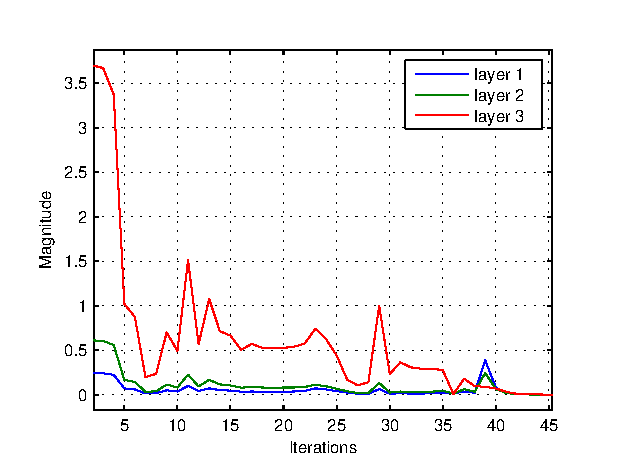
\includegraphics{figures/meanGradMag}}
			\end{figure}
		\end{minipage}
	\end{itemize}

	\end{frame}
	
\section{Unsupervised greedy layer-wise pre-training}
	
	
	\begin{frame}[t]{Unsupervised greedy layer-wise pre-training}
	
		\begin{itemize}
			\item Train the Deep Neural Network layer by layer (Hinton, Bengio)	
			\item Truncate network after first layer		
		\end{itemize}

		\begin{minipage}[t]{0.48\linewidth}
			\begin{figure}
				\psfrag{A}{$\underline{x}_k$}
				\psfrag{B}{$\underline{\hat{y}}_k$}
				\psfrag{I}{Input}
				\psfrag{C}{Coding}
				\psfrag{O}{Output}						
				\scalebox{0.7}{\includegraphics{figures/layerTraining01}}
			\end{figure}
		\end{minipage}
		
	\end{frame}
	
		\begin{frame}[t]{Unsupervised greedy layer-wise pre-training}
		
		\begin{minipage}[t]{0.48\linewidth}
			\begin{figure}
				\psfrag{A}{$\!\!\! \underline{a}_k^{(1)} = \underline{x}_k$}
				\psfrag{B}{$\underline{\hat{a}}_k^{(1)}$}
				\psfrag{I}{Input}
				\psfrag{C}{Coding}
				\psfrag{O}{Output}
				\psfrag{R}{Reconstruction}
				\psfrag{S}{Auto-Encoder}
				\psfrag{W}{${\bf W}^{(1)}$}
				\psfrag{V}{${\bf W}^{(1)T}$}
				\psfrag{E}{$\underline{b}_{enc}^{(1)}$}				
				\psfrag{F}{$\underline{b}_{rec}^{(1)}$}
				\scalebox{0.7}{\includegraphics{figures/layerTraining02}}
			\end{figure}
		\end{minipage}\hfill
		\begin{minipage}[t]{0.48\linewidth}
			\begin{itemize}					
				\item Reconstruction error
					\begin{equation}
						J_{AE} = \sum_{\forall k} \frac{1}{2} ||\underline{a}^{(1)}_k - \hat{\underline{a}}^{(1)}_k||^2 \nonumber
					\end{equation}				
				\item Small hidden layer: Learned subspace similar to PCA for linear activation $\underline{\Phi}(\cdot)$
			\end{itemize}
		\end{minipage}
		\vspace{1cm}
		\begin{itemize}
		\item Activation of the output layer
			$ \hat{\underline{a}}^{(1)}_k = \underline{\Phi} \left (  {\bf W}^T \underline{\Phi} \left ( {\bf W} \underline{x}_k  + \underline{b}_{enc} \right ) + \underline{b}_{rec} \right )$
		\end{itemize}
	\end{frame}
	
	\begin{frame}[t]{Unsupervised greedy layer-wise pre-training}
	\textcolor{blue}{\Large Force non-trivial solution}		
				\begin{itemize}
				\item Reduce number of hidden neurons
				\item Regularization
					\begin{equation}
						J_{reg} = ||{\bf W}||_F^2 
					\end{equation}
				\item Sparsity constraint
					\begin{eqnarray}
						\hat{\rho} &=& \frac{1}{m} \sum_{\forall k} [\underline{a}_k^{(2)}]_n \\
						J_{sp} &=& \sum_{\forall n} \mathrm{KL}(\rho||\hat{\rho}_n) \\
						\mathrm{KL}(\rho||\hat{\rho}_n) &=& \rho \log \frac{\rho}{\hat{\rho}_n}+ (1-\rho) \log \frac{1-\rho}{1-\hat{\rho}_n}
					\end{eqnarray}
				\item Overall cost
				\begin{equation}
					J = J_{AE}+ \lambda J_{reg} + \beta J_{sp}
				\end{equation}
					
				\end{itemize}
	\end{frame}
	
		
	\begin{frame}[t]{Unsupervised greedy layer-wise pre-training}
		\begin{itemize}
				\item Propagate input to second layer
				 \begin{equation}
					\underline{a}^{(2)}_k = \underline{\Phi} \left ( {\bf W}^{(1)} \underline{a}_k^{(1)}  + \underline{b}^{(1)} \right ) \nonumber
					\end{equation}
				\item Do pre-training of second layer
				\item ...
		\end{itemize}
		
			\begin{figure}
				\psfrag{A}{$\underline{a}_k^{(2)}$}
				\psfrag{B}{$\underline{\hat{a}}_k^{(2)}$}
				\psfrag{I}{Input}
				\psfrag{C}{Coding}
				\psfrag{O}{Output}
				\psfrag{R}{Reconstruction}
				\psfrag{S}{Stacked Auto-Encoder}
				\psfrag{W}{${\bf W}^{(2)}$}
				\psfrag{V}{${\bf W}^{(2)T}$}
				\psfrag{E}{$\underline{b}_{enc}^{(2)}$}				
				\psfrag{F}{$\underline{b}_{rec}^{(2)}$}
				\scalebox{0.7}{\includegraphics{figures/layerTraining03}}
			\end{figure}
		
				
	\end{frame}
	
			
	\begin{frame}[t]{Unsupervised greedy layer-wise pre-training}
		\begin{itemize}
				\item Add randomly initialized classification layer
				\item Perform dicriminative fine tuning, optimizing over weights and bias 
					terms of each stage
		\end{itemize}
		\begin{figure}
				\psfrag{A}{$\underline{x}_k$}
				\psfrag{B}{$\underline{\hat{y}}_k$}
				\psfrag{I}{Input}
				\psfrag{O}{Output}
				\psfrag{R}{Reconstruction}
				\psfrag{S}{Deep Neural Network}
				\scalebox{0.7}{\includegraphics{figures/layerTraining04}}
			\end{figure}
				
	\end{frame}

\section{Experiments}
	\subsection{Auto-Encoder for data compression}
	
	\begin{frame}[t]{Data compression}
	
	\begin{minipage}[t]{0.48\linewidth}
	\textcolor{blue}{\Large Experimental Setup}	
	\begin{itemize}
			\item Take 10 gray scale images
			\item Extract non-overlapping 8x8 patches
			\item Train Auto-Encoder for compression		
			\item Setup of the Auto-Encoder			
				\begin{itemize}
					\item 1 hidden layer $[64, 25, 64]$
					\item Training with 10.000 randomly selected patches
					\item LBFGS for optimization
					\end{itemize}
		\end{itemize}
	\end{minipage}\hfill
	\begin{minipage}[t]{0.48\linewidth}
		\begin{figure}
		\psfrag{A}{$\underline{x}_k$}
		\psfrag{B}{$\underline{\hat{x}}_k$}
		\psfrag{C}{Single stage Auto-Encoder}
		\psfrag{D}{Grayscale image}
			\scalebox{0.6}{\includegraphics{figures/compressionStructure}}
		\end{figure}
	\end{minipage}
	
	\end{frame}
	
	\begin{frame}[t]{Data compression}
	
	\begin{minipage}[t]{0.48\linewidth}
	\textcolor{blue}{\Large Original}	
		\begin{figure}
			\scalebox{0.4}{\includegraphics{figures/texture}}
		\end{figure}
	\end{minipage}\hfill
	\begin{minipage}[t]{0.48\linewidth}
	\textcolor{blue}{\Large Reconstructed}
		\begin{figure}
			\scalebox{0.4}{\includegraphics{figures/textureRec}}
		\end{figure}		
	\end{minipage}
	
	\end{frame}
	
	\begin{frame}[t]{Data compression}
	
	\begin{minipage}[t]{0.48\linewidth}
	\textcolor{blue}{\Large Learned features}	
			\begin{figure}
				\raggedleft
				\scalebox{0.5}{\includegraphics{figures/extractedFeatures}}
			\end{figure}

	\end{minipage}\hfill
	\begin{minipage}[t]{0.48\linewidth}
	\begin{itemize}
		\item Visualization
			\begin{itemize}
				\item Plot row vectors of ${\bf W}^{(1)}$, because:
			\end{itemize}
			\begin{equation}
				\underline{z}^{(2)}_k = {\bf W}^{(1)} \underline{x}_k + \underline{b}^{(1)} \nonumber
			\end{equation}

		\item The features are
		\begin{itemize}
			\item Corner features
			\item Edge features
			\item Texture features
		\end{itemize}
	\end{itemize}
	\end{minipage}
	
	\end{frame}
	
	\subsection{dNN for digit recognition}
	
	\begin{frame}[t]{Digit Recognition}
	
	\begin{minipage}[t]{0.48\linewidth}
	\textcolor{blue}{\Large Experimental Setup}	
	\begin{itemize}
			
			\item Using MNIST data base 
				\begin{itemize}
					\item 60.000 binar training images
					\item 10.000 binar test images
					\item 28x28 pixels
				\end{itemize}
							
			\item Setup of the dNN			
				\begin{itemize}
					\item 4 hidden layers $[784, 500, 200, 100, 10, 4]$
					\item Sigmoid activation function in all layers
					\item Tied-weights during layer-wise pre-training
					\item Cost / gradient calculation with all 60.000 training sets
					\item LBFGS for optimization 
				\end{itemize}
		\end{itemize}
	\end{minipage}\hfill
	\begin{minipage}[t]{0.48\linewidth}
		\only<1-1>{
		\textcolor{blue}{\Large First stage features}
		\begin{figure}
			\raggedleft
				\scalebox{0.5}{\includegraphics{figures/featuresMNIST}}
			\end{figure}}
	\end{minipage}
		
	\end{frame}
	
	
	\begin{frame}[t]{Digit Recognition}
			
		\begin{minipage}[t]{0.48\linewidth}
			\textcolor{blue}{\Large Last stage features}
			\begin{figure}
				\includegraphics{figures/digitPrototypes}
			\end{figure}
	%		\begin{equation}
%				\left [ \underline{x}^{(ol)} \right ]_n = \arg \max_{\underline{x}, s.t ||\underline{x}|| = 1} \left [ \underline{a}^{(ol)} \right ]_n \nonumber
%			\end{equation}
		\end{minipage}\hfill			
		\begin{minipage}[t]{0.48\linewidth}
		\textcolor{blue}{\Large Result}
			\begin{itemize}
				\item Clustering into 16 groups
				\item Learned representations are prototypes of handwritten digits			
				\item Recognition rate after discarding the last layer and performing
					discriminative fine tuning $98.2 \%$
			\end{itemize}
		\end{minipage}
	\end{frame}
	
	\subsection{Auto-Encoder for image reconstruction}

	\begin{frame}[t]{Auto-Encoder for image reconstruction}
	\textcolor{blue}{\Large Experimental Setup}	
	
	\begin{minipage}[t]{0.48\linewidth}
		\begin{figure}
		\psfrag{A}{$\underline{\tilde{x}}_k$}
		\psfrag{B}{$\underline{\hat{x}}_k$}
		\psfrag{C}{Single stage Auto-Encoder}
		\psfrag{D}{Distorted digits}
			\scalebox{0.6}{\includegraphics{figures/reconstructionStructure}}
		\end{figure}
	\end{minipage}\hfill
	\begin{minipage}[t]{0.48\linewidth}
		\begin{itemize}
		\uncover<1->{	
			\item Using MNIST data base 
			\item Adding random distortion which flips values at arbitrary positions
			$\underline{\tilde{x}}_k = \underline{x}_k + \underline{w}$
			}
			
			\uncover<1->{	
			\item Setup of the Auto-Encoder			
				\begin{itemize}
					\item 1 hidden layer $[784, 196, 784]$
					\item Sigmoid activation function in all layers
					\item Tied-weights
					\item Cost / gradient calculation with all 60.000 training sets
					\item LBFGS for optimization 
				\end{itemize}}
		\end{itemize}
	\end{minipage}
		
	\end{frame}
	
	\begin{frame}[t]{Auto-Encoder for image reconstruction}
	\textcolor{blue}{\Large Results}	
	
	\begin{minipage}[t]{0.48\linewidth}
		\begin{figure}
			\scalebox{0.6}{\includegraphics{figures/distorted01}}
		\end{figure}
	\end{minipage}\hfill
	\begin{minipage}[t]{0.48\linewidth}
		\begin{figure}
			\scalebox{0.6}{\includegraphics{figures/reconstruction01}}
		\end{figure}
	\end{minipage}
	
	Quadratic error:
	\begin{eqnarray}
		e_1 &=& \frac{1}{NL} \sum_{k = 1}^N || \underline{x}_k - \tilde{\underline{x}}_k ||^2 = 0.0873 \nonumber \\
		e_2 &=& \frac{1}{NL} \sum_{k = 1}^N || \underline{x}_k - \hat{\underline{y}}_k ||^2 = 0.0158 \nonumber 
	\end{eqnarray}	
		
	\end{frame}
	
	\begin{frame}[t]{Auto-Encoder for image reconstruction}
	\textcolor{blue}{\Large Results}	
	
	\begin{minipage}[t]{0.48\linewidth}
		\begin{figure}
			\scalebox{0.6}{\includegraphics{figures/distorted02}}
		\end{figure}
	\end{minipage}\hfill
	\begin{minipage}[t]{0.48\linewidth}
		\begin{figure}
			\scalebox{0.6}{\includegraphics{figures/reconstruction02}}
		\end{figure}		
	\end{minipage}
		
	Quadratic error:
	\begin{eqnarray}
		e_1 &=& \frac{1}{NL} \sum_{k = 1}^N ||\underline{x}_k - \tilde{\underline{x}}_k ||^2 = 0.2038 \nonumber \\
		e_2 &=& \frac{1}{NL} \sum_{k = 1}^N || \underline{x}_k - \hat{\underline{y}}_k ||^2 = 0.0239 \nonumber 
	\end{eqnarray}		
		
	\end{frame}
	
	\begin{frame}[t]{Auto-Encoder for image reconstruction}
		\textcolor{blue}{\Large Why this works (Vincent et al. 2010)}	
		\begin{figure}
			\includegraphics{figures/denoising}
		\end{figure}
		\begin{itemize}
			\item Auto-Encoder captures structure of input distribution
			\item Learns to map from low-probability regions to lower-dimensional
				high-probability regions
		\end{itemize}
	\end{frame}
	
\section{Summary}
	\begin{frame}[t]{Auto-Encoder for image reconstruction}
	\begin{itemize}
		\item Deep Architectures can bridge the gap between feature engineering and
			classification (representation learning)
		\item Deep Architectures can learn hierarchical abstractions from high-dimensional
			raw data and therefore enable non-local learning
		\item Greedy layer-wise pre-training results in an initialization of the network
			near a good local minima of the cost function
		\item Only unlabeled data is used during pre-training
		\item Stacked Auto-Encoders can be used for reconstruction of noisy data
			(Maybe even for reconstruction of MR-Images??)
	\end{itemize}	
	\end{frame}

\end{document}
